%---------------------导言区---------------------------%
\documentclass[12pt,a4paper,UTF8]{ctexart}
	%10pt:正文字体为12pt,缺省为10pt;各层级字体大小会根据正文字体自动调整
	%a4paper:纸张大小a4;
	%UTF8:中文要求
\usepackage{geometry}%用于设置上下左右页边距
	\geometry{left=2.5cm,right=2.5cm,top=3.2cm,bottom=2.8cm}
\usepackage{xeCJK,amsmath,paralist,enumerate,booktabs,multirow,graphicx,subfig,setspace,listings,lastpage,hyperref,amssymb,upgreek}
	%xeCJK:中文字体(如楷体,作者和机构需要用到)的设置
	%amsmath:数学公式
	%paralist,enumerate:自定义项目符号
	%booktabs:三线图,论文常用的表格风格
	%multirow:复杂表格
	%graphicx,float: 插入图片
	%subfig:并排排版图片、竖向排版图片
	%setspace:设置行间距等功能
	\setlength{\parindent}{2em}%正文首行缩进两个汉字
	%listings:用于排版各种代码;比如matlab的代码
	\lstset{language=Matlab}%matlab代码
	%lastpage:获取总页数;
	%hyperref:超链接,和lastpage搭配.
\usepackage{fancyhdr}
	%fancyhdr:一个很强大的宏包,用于自定义设计页面风格并命名以供调用。
	\pagestyle{fancy}
	\rhead{实验 B0.1 参考文献的检索和管理}
	\lhead{基础物理实验\uppercase\expandafter{\romannumeral2}实验报告}
	\cfoot{Page \thepage/\pageref{LastPage}}  %当前页\总页数
		%分别是右页眉、左页眉、中页脚、右页脚
	\renewcommand{\headrulewidth}{0.4pt}
	\renewcommand{\theenumi}{(\arabic{enumi})}
	\setlength\headheight{15pt}

% \setCJKmainfont{FZShuSong-Z01S}[ItalicFont=FZKai-Z03S, BoldFont=FZHei-B01S]
%中文字体设置:使用开源字体方正书宋,方正楷体和方正黑体



%%%%%%%%%%%%%%%%%%%%%%%%%正文开始%%%%%%%%%%%%%%%%%%%%%%%%%%

\begin{document}

%%begin-------------------标题与信息-----------------------%%

%%标题
\begin{center}
\LARGE\textbf{实验 B0.1 参考文献的检索和管理}
\end{center}

%%信息
\begin{doublespacing}
	%doublespacing:手动两倍行距
	\centering
	\begin{tabular}{lr}
	 & \\
	{\CJKfontspec{方正楷体简体} 学院:中山医学院} & {\CJKfontspec{方正楷体简体} 年级、专业:2020级临床医学(长学制)} \\
	{\CJKfontspec{方正楷体简体} 实验人姓名、学号:莫润冰~20980131} & {\CJKfontspec{方正楷体简体}}\\
	{\CJKfontspec{方正楷体简体} 实验时间:2021年9月16日~星期四~上午} & {\CJKfontspec{方正楷体简体} 室温:27$^{\circ}$C~ 相对湿度:53\%}
	\end{tabular}
\end{doublespacing}

%%end-------------------标题与信息-----------------------%%


\subsection*{【实验目的】}
	%*表示不带上小节本身应有的1.1,下面的subsubsection*也是一样
%%自定义项目符号之(1)(2)(3)
	\begin{enumerate}[(1)]
		\item 学习利用 Endnote 软件检索和管理科技文献。
		\item 学习利用 Endnote 与 Microsoft Word 配合写作的方法。
	\end{enumerate}

\subsection*{【实验设备】}
安装了 Microsoft Word 和 Endnote 软件的计算机。可自带笔记本电脑完成
实验。

\subsection*{【实验原理】}
参考文献的检索、管理、阅读和引用是学术研究工作的一项重要内容。按照
最新颁布的国家标准 GB/T 7714-2015《信息与文献 参考文献著录规则》中的定
义,参考文献是指“为撰写或编辑论文和著作而引用的有关文献信息资源”[1],
包括专著、期刊论文、学位论文、专利、技术标准、网页、音像资料等数十种类
型。参考文献的质量是评价学术成果质量的一个重要指标。本科阶段的学生,有
必要尽快掌握参考文献的检索、管理和正确引用方法。

在利用 Microsoft Word 进行科技论文、学位论文和实验报告的写作时,如
果文献较少,可以利用软件中“引用”菜单中的“插入引文”功能完成参考文献
的引用和自动排序,但参考文献数量较大时,利用专业的参考文献管理软件可极
大地提高工作效率和准确率。目前,常用的参考文献管理软件有许多种,如
Endnote、NoteExpress、NoteFirst、CNKI-eLearning、Citavi、Mendeley、Zotero 等。
这些软件各有特色,如支持哪种操作系统,是否有单机版和网络版,支持哪种浏
览器,免费版还是收费版等,建议使用者根据自己的实际情况,选择其中至少一
种软件并熟练掌握其使用方法。

本实验将以 Endnote 为例[2],说明参考文献检索和管理的基本方法。Endnote
是由 Thomson Research Soft 开发的文献管理软件系统,由于该软件和 Web of
Science 数据库同属于 Clarivate Analytics 公司的产品,兼容性较好,并支持将图、
表、公式等作为参考文献,在论文写作时方便调用,故目前在科研人员中使用较
为广泛。该软件最新的版本为 X8 版,可在系统中直接连接约 6000 个数据库进行
约 50 种类型文献信息的检索,支持 6800 多种参考文献的输出格式,并内置了约
300 种期刊的投稿模板。Endnote X8 全功能单机版的价格较高,初学者可安装免
费的 Basic 版本,但使用的时候需要连接 Internet。相关软件和学习资料可到官网
http://www.endnote.com/downloads 处下载。文献[3]可作为 Endnote 使用的入门
训练手册,更深入的学习可参阅文献[4]。

Endnote 的一些重要概念:


\paragraph*{(1)} 
Endnote 以图书馆(library 文件,后缀名.enl)的格式管理参考文献,
该文件与同名的文件夹配合使用,分享文献的时候需要同时拷贝文件夹。参考文
献的类型名称和每个栏目的作用可参阅文献[5]。
\paragraph*{(2)} 
Endnote 有 Local Library Mode、 Online Search Mode、Integrated
Library \& Online Search Mode 三种工作模式。
\paragraph*{(3)} 
Endnote 可利用“Import”功能导入 pdf 文件,自动生成 pdf 文件的
参考信息。也可以根据已有的参考信息,通过“Find Full Text”功能下载全文。
\paragraph*{(4)} 
使用单机版 Endnote 时参考文献需要保存在本地计算机,若使用网
络位置会导致系统崩溃。
\paragraph*{(5)} 
Endnote 使用中涉及 Import Filter(后缀.enf)、Output Style(后缀.ens)、
Connection file(后缀.enz)和 template(后缀.dot)几种类型的重要文件:

Import Filters:从其他软件的参考文献或 pdf 文件转换到 endnote 格式时需
要使用的转换规则文件。

Output Styles:参考文献输出格式文件,系统内置的均为外文期刊。中文期
刊要求的 GB/T 7714-2015 格式文件需要自己重新编写。

Connection files:数据库连接文件,包含数据库检索的必要信息,如服务器
名称、地址、端口,检索信息的类型、内容标签等。

Templates:论文模板文件,定义的投稿文章的内容、栏目、字数限制、图
表格式等。


\subsection*{【实验内容及步骤】}
1.安装 Endnote X8 试用版或 Basic 版,并在 Microsoft Word 中调用加载项。

注:实验技术人员已在实验室的计算机上完成了安装。\\

2.了解 Endnote 工作界面,学习 Endnote 基本使用方法。

参阅文献《Endnote Menus Reference Guide》[3]和《The Little Endnote How-to Book》
[6]。\\

3. 建立参考文献库,输入若干参考文献

	\begin{enumerate}[(1)]
			\item 文献库名称为“基础物理实验”(或 GeneralPhysicsLab)。
			\item 手工输入教材后表列的至少 6 条参考文献内容,包含书籍、论文、标
			准等几种类型。
			\item 用 Endnote 的“import file”功能导入 pdf 文件,自动生成参考文献信
			息。
			\item 网上检索参考文献并保存 10 条信息。
			
			例 1:检索 Web of Science 数据库,检索 title 包含“pendulum”的文
			献,需具有对该数据库的检索权限。或通过中山大学图书馆的电子期
			刊页进入数据库的检索页面,基于浏览器检索后选择 10 条文献导入
			Endnote。

			例 2:自己选择感兴趣的内容进行检索,如 CUPT 竞赛内容、广东物
			理实验设计大赛内容、本科生科研训练项目内容、课题组导师要求的
			内容等。
			\item 用 Endnote 的“Find Full Text…”功能补齐参考文献对应的 pdf 文件。			
	\end{enumerate}

	4. 建立分组(Groups set 和 Groups)

	\begin{enumerate}[(1)]
		\item 建立三个 Groupsset,名称分别为“基础物理实验 I”、“基础物理实验
		II”和“基础物理实验 III”。
		\item 在“基础物理实验 III”中建立分组,名称分别为“ExpC2”、“ExpC3”…
		等,包括本学期所有实验的编号。
		\item 建立自己感兴趣的其他分组。
		\item 根据个人学习进度,将检索到的文献分配至不同的分组中。右键点击
		需要分组的文献,在弹出菜单中选择“Add Referencesto”进行分配。
	\end{enumerate}

	5. 编写符合 GB/T 7714-2015 标准的 Output style 文件
	
	\begin{enumerate}[(1)]
		\item 选择“Tools>Output Styles>Numbered”,再选择“Tools>Output Styles> Edit
		Numbered”编辑 Output Style 文件,并用名称“GB-T7714-2015.ens”
		另存。
		\item 入门学习阶段,主要修改该文件中“Citations”和“Bibliography”中的
		templets 内容,根据 GB/T 7714-2015 标准修改其中的括号、标点、参
		考信息内容、排列顺序等。保存并退出 styles 文件的编辑。
		\item 主界面中选择“Tools>Output Styles> GB/T 7714-2015”,分别点选书籍、
		论文、标准等不同类型的参考文献条目,在右侧的“preview”窗口中
		检查文献显示的格式是否符合标准。
		\item 如果不符合,则重新编辑“GB/T 7714-2015”style 文件,直至所有的显
		示都符合标准。
	\end{enumerate}

	6. Endnote 和 Word 配合,撰写实验报告或课程论文

	结合同学自己的学习进度进行操作,报告或论文的内容不同,或自带其
	他需要编写参考文献的文章。

	\begin{enumerate}[(1)]
		\item 插入参考文献。打开 Endnote 和 Word,在 word 中将光标移动至需要
		插入参考文献的地方,在 Endnote 中打开参考文献库文件,选择输出
		格式文件(本实验中为 GB/T 7714-2015),点选需要插入的文献,点击
		“Tools>Cite While You Write>Insert Selected Citation(s)”插入文献。则
		在文章末尾自动生成符合 GB/T 7714-2015 标准的参考文献列表,编号
		按文献在文章中引用的先后顺序自动排列。
		\item 修改和调整参考文献,并调整格式,直至完成实验报告或课程论文。
	\end{enumerate}

\subsection*{【实验结果】}


\begin{figure*}[htbp]
	\centering
	\subfloat[文献分组情况]{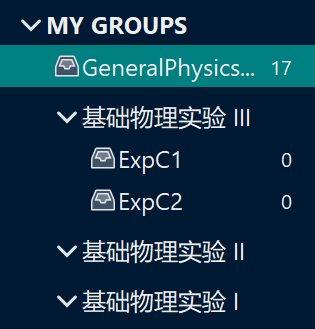
\includegraphics[width=0.4\textwidth]{img//library.png}}
	\subfloat[组内文献目录]{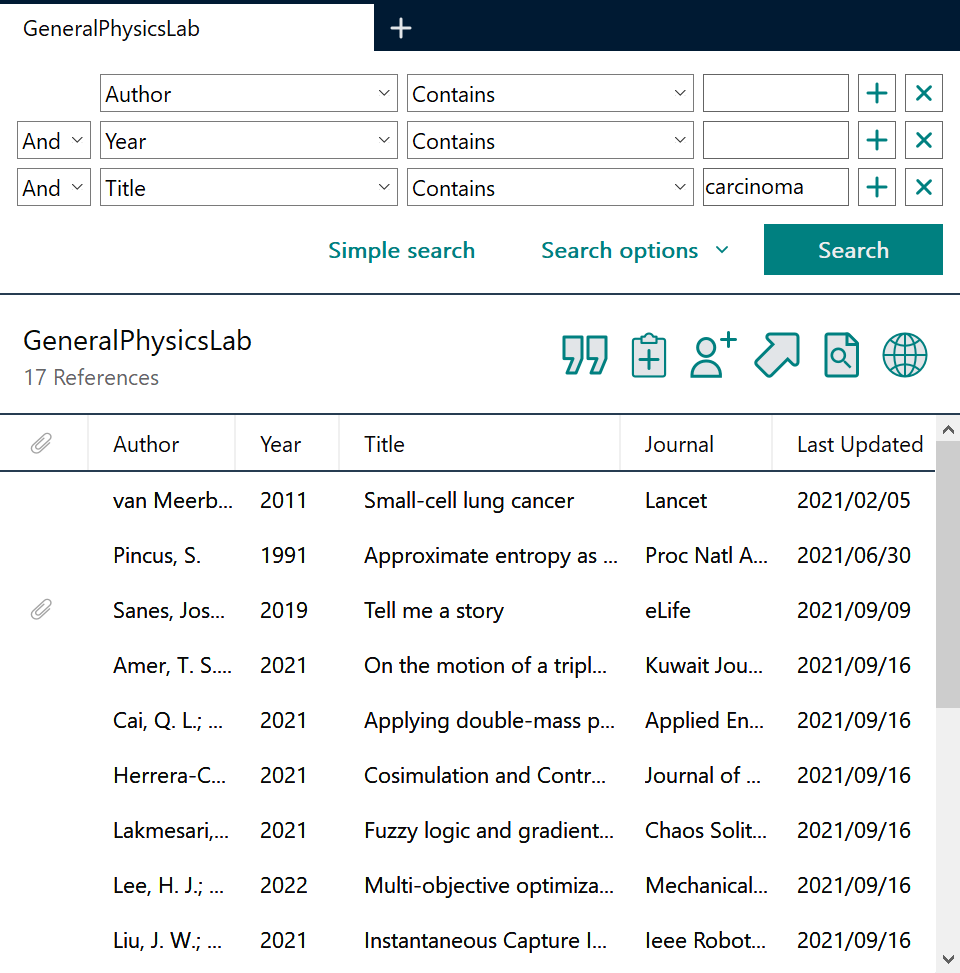
\includegraphics[width=0.4\textwidth]{img//content.png}}

	\subfloat[单个文献详细信息]{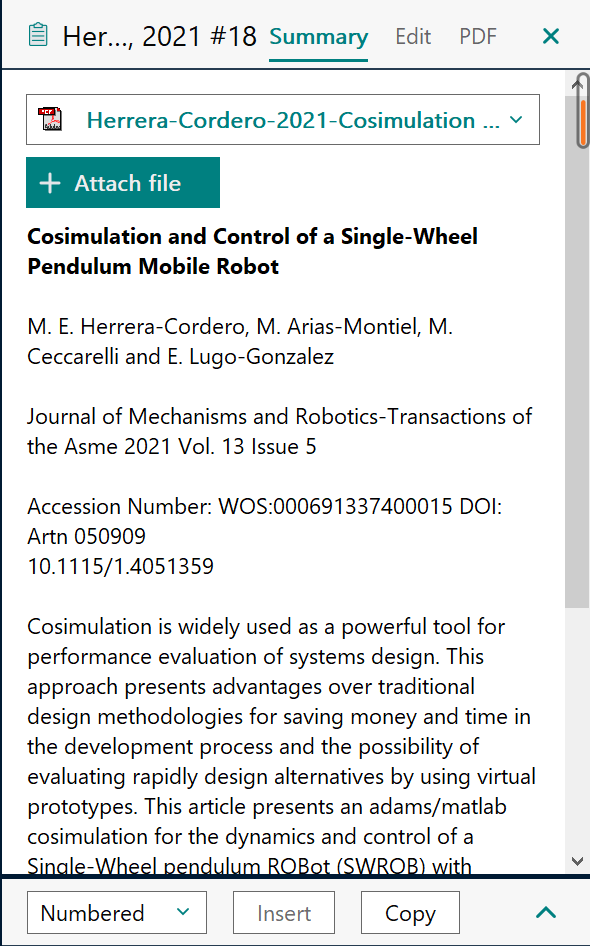
\includegraphics[width=0.4\textwidth]{img//detail.png}}
	\subfloat[参考文献格式设置界面]{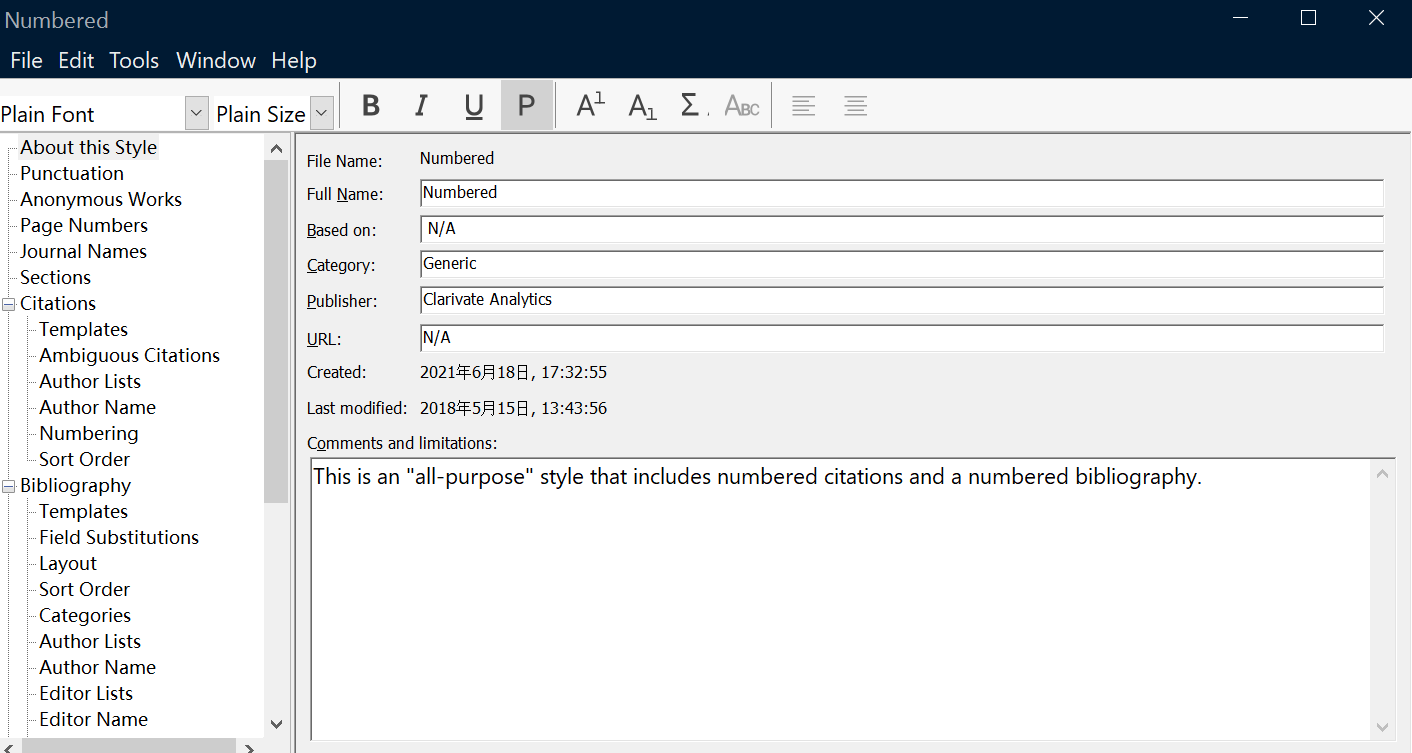
\includegraphics[width=0.4\textwidth]{img//outputstyle.png}}
	\caption{文献管理}
\end{figure*}


\begin{figure}[htbp]
	\centering
	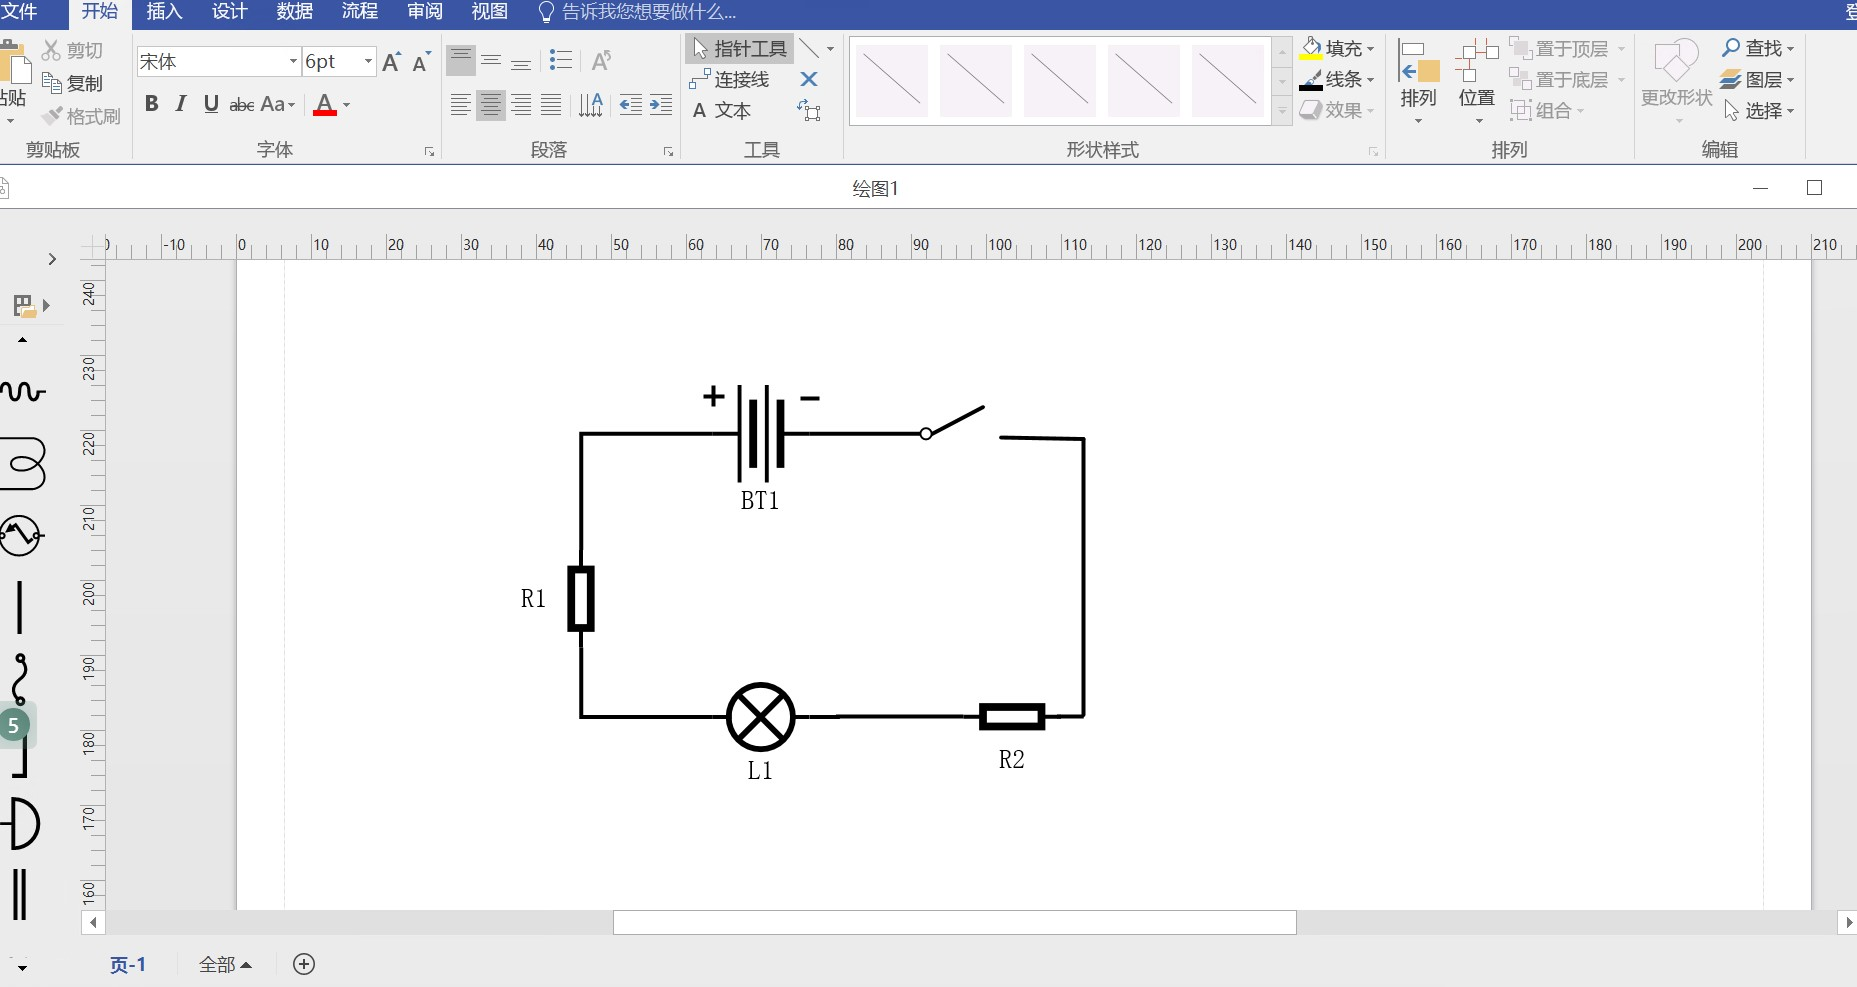
\includegraphics[width=0.8\textwidth]{img//fig2.jpg}
	\caption{绘图界面}
\end{figure}



\begin{figure}[htbp]
	\centering
	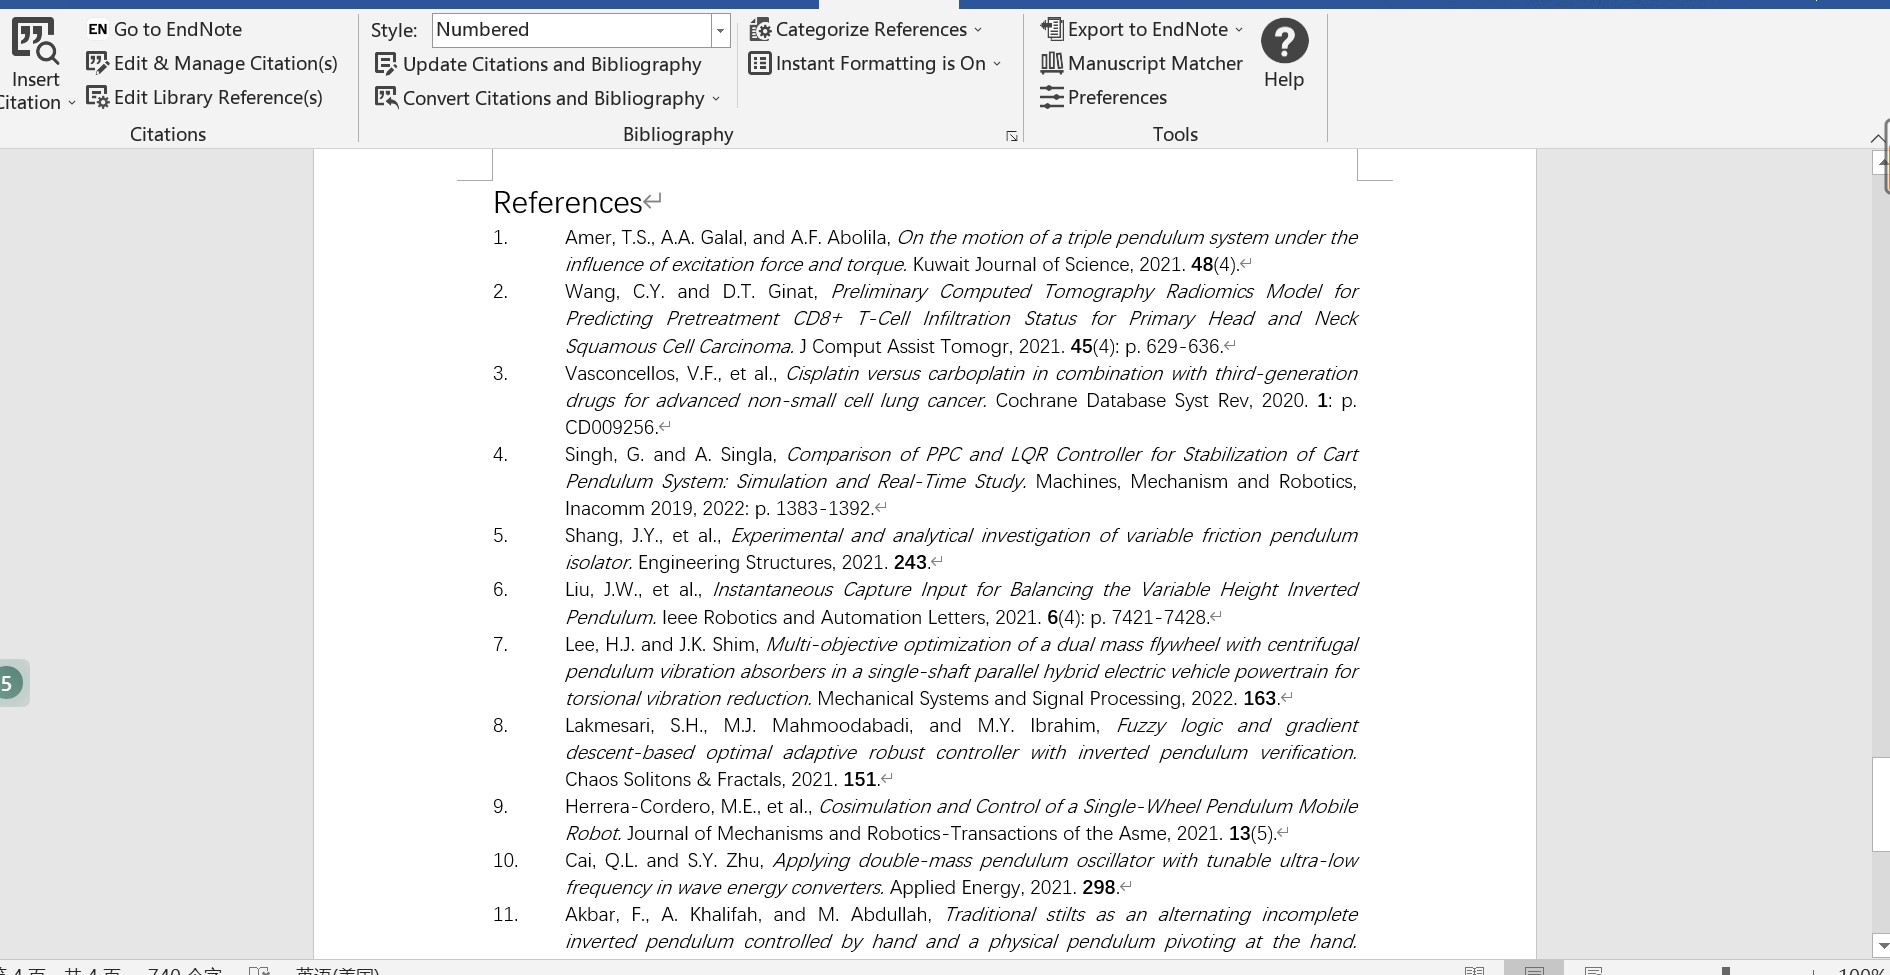
\includegraphics[width=0.8\textwidth]{img//import.jpg}
	\caption{文献导入界面}
\end{figure}



\subsubsection*{公式输入}

\begin{gather}
	f_r=6\pi a \eta v_g   \\
	m=4 \pi a^{3} \rho / 3
\end{gather}

\begin{equation}
	\eta^{\prime}=\eta /[1+b /(p a)]
\end{equation}

\[e=(1.60217733 \pm 0.00000049) \times 10^{-19} \mathrm{C}\]

\[\left\{%\left和\right配合使用,可以得到大小匹配的各种括号
\begin{aligned}
&C_{1} \cdot \frac{d U_{C_{1}}}{d t}=\frac{1}{R_{1}} \cdot(u_{C_{2}}-u_{C_{1}})-f(u_{R_{N}}) \\
&C_{2} \cdot \frac{d U_{C_{2}}}{d t}=i_{L}-\frac{1}{R_{1}} \cdot(u_{C_{2}}-u_{C_{1}}) \\
&L \cdot \frac{d i_{L}}{d t}=-U_{C_{2}}
\end{aligned}
\right.
\]



\subsection*{【思考题】}

	\subsubsection*{1. 检索若干种参考文献管理软件的说明文件,对比它们的优缺点。}
	答:EndNote界面简洁,交互按钮少,容易上手;而NoteExpress交互界面复杂,较难上手。
	EndNote适合英文文献的在整理;而NoteExpress相对适配中文文献。
	EndNote数据库强大,有PubMed、Web of Science 等,NoteExpress数据库相对没有那么丰富。
	在操作方面,EndNote可以将文献拖拽至相应文件夹,操作方便;而NoteExpress不可以。

	\subsubsection*{2. 查阅帮助文件,实现参考文献的多人共享,网络与本地文献同步等其他功能。}
	
	\begin{figure}[htbp]
		\centering
		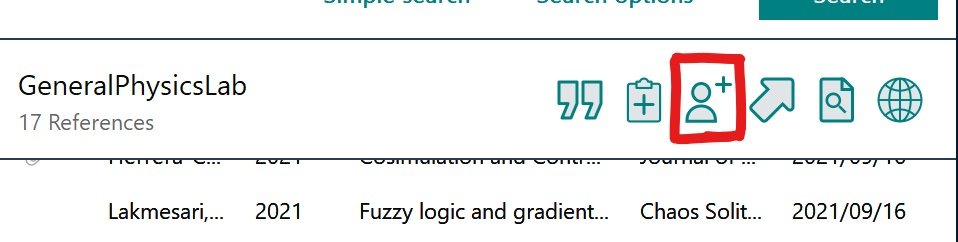
\includegraphics[width=0.8\textwidth]{img//share.jpg}
		\caption{参考文献的多人共享}
	\end{figure}


	
	图6中框出区域即为共享按钮。

	\newpage
	\subsection*{附录}

	\begin{figure}[htbp]
		\centering
		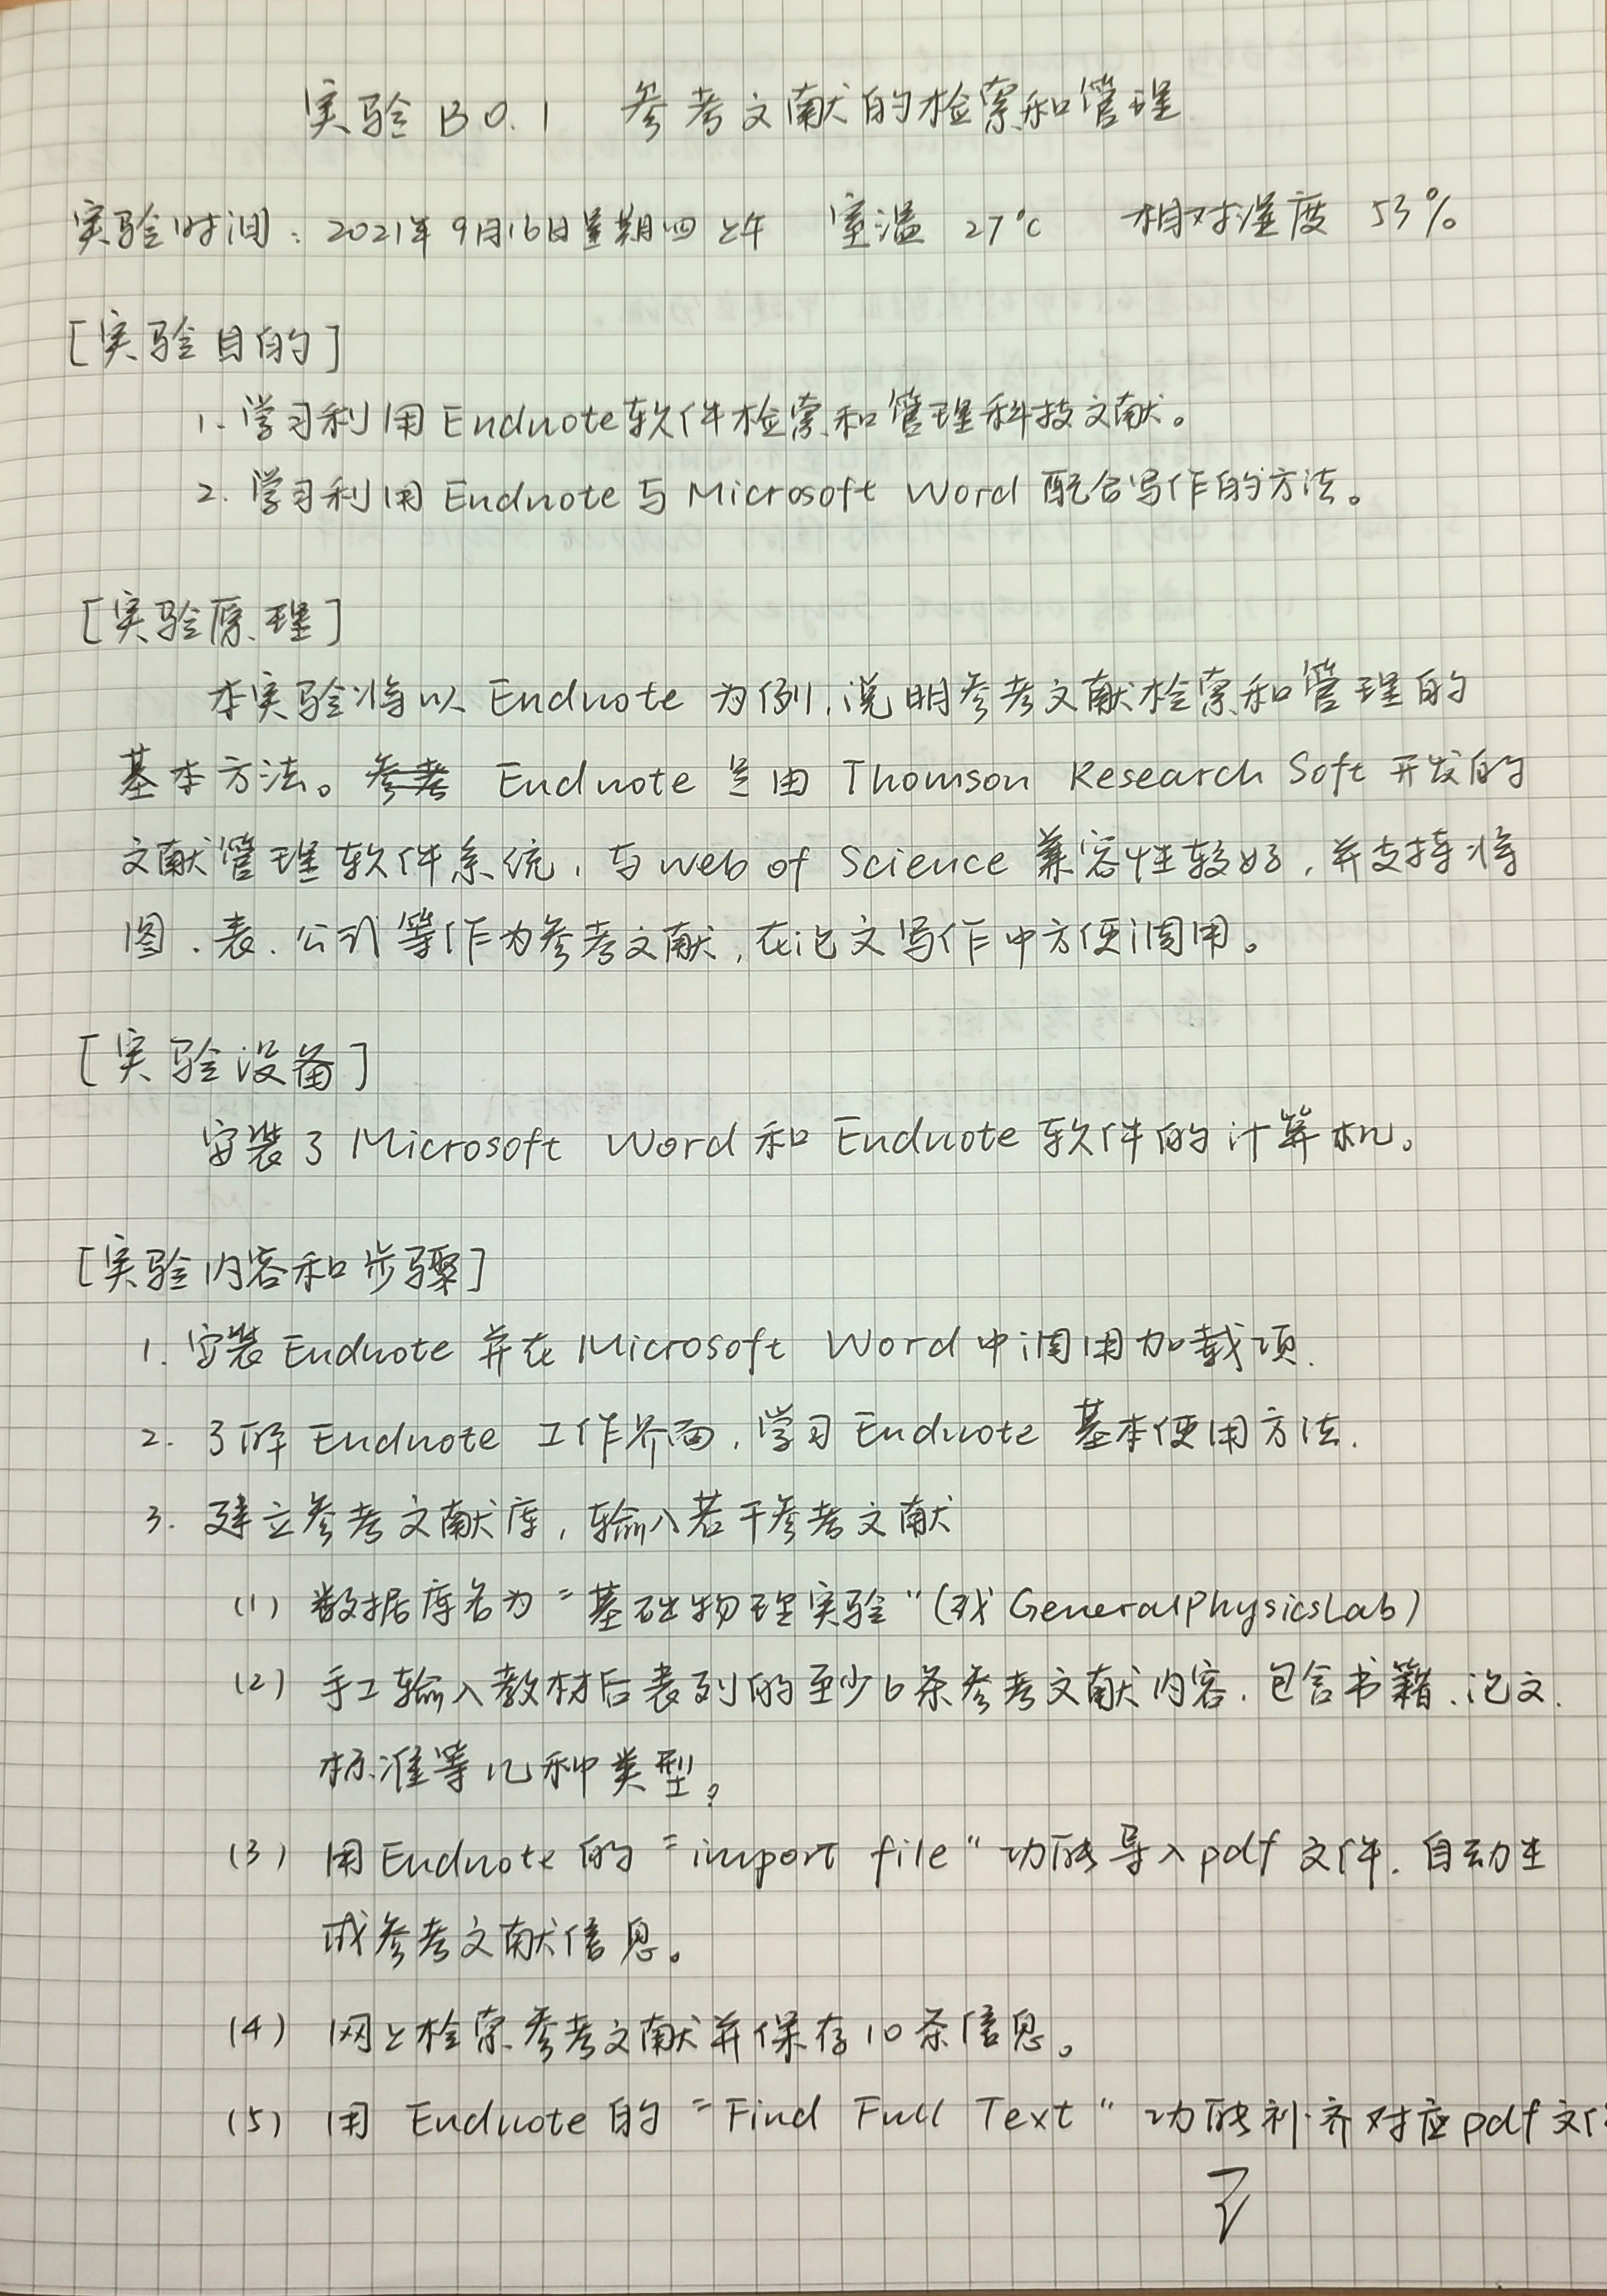
\includegraphics[width=0.8\textwidth]{img//preview1.jpg}
	\end{figure}
	\begin{figure}[htbp]

		\centering
		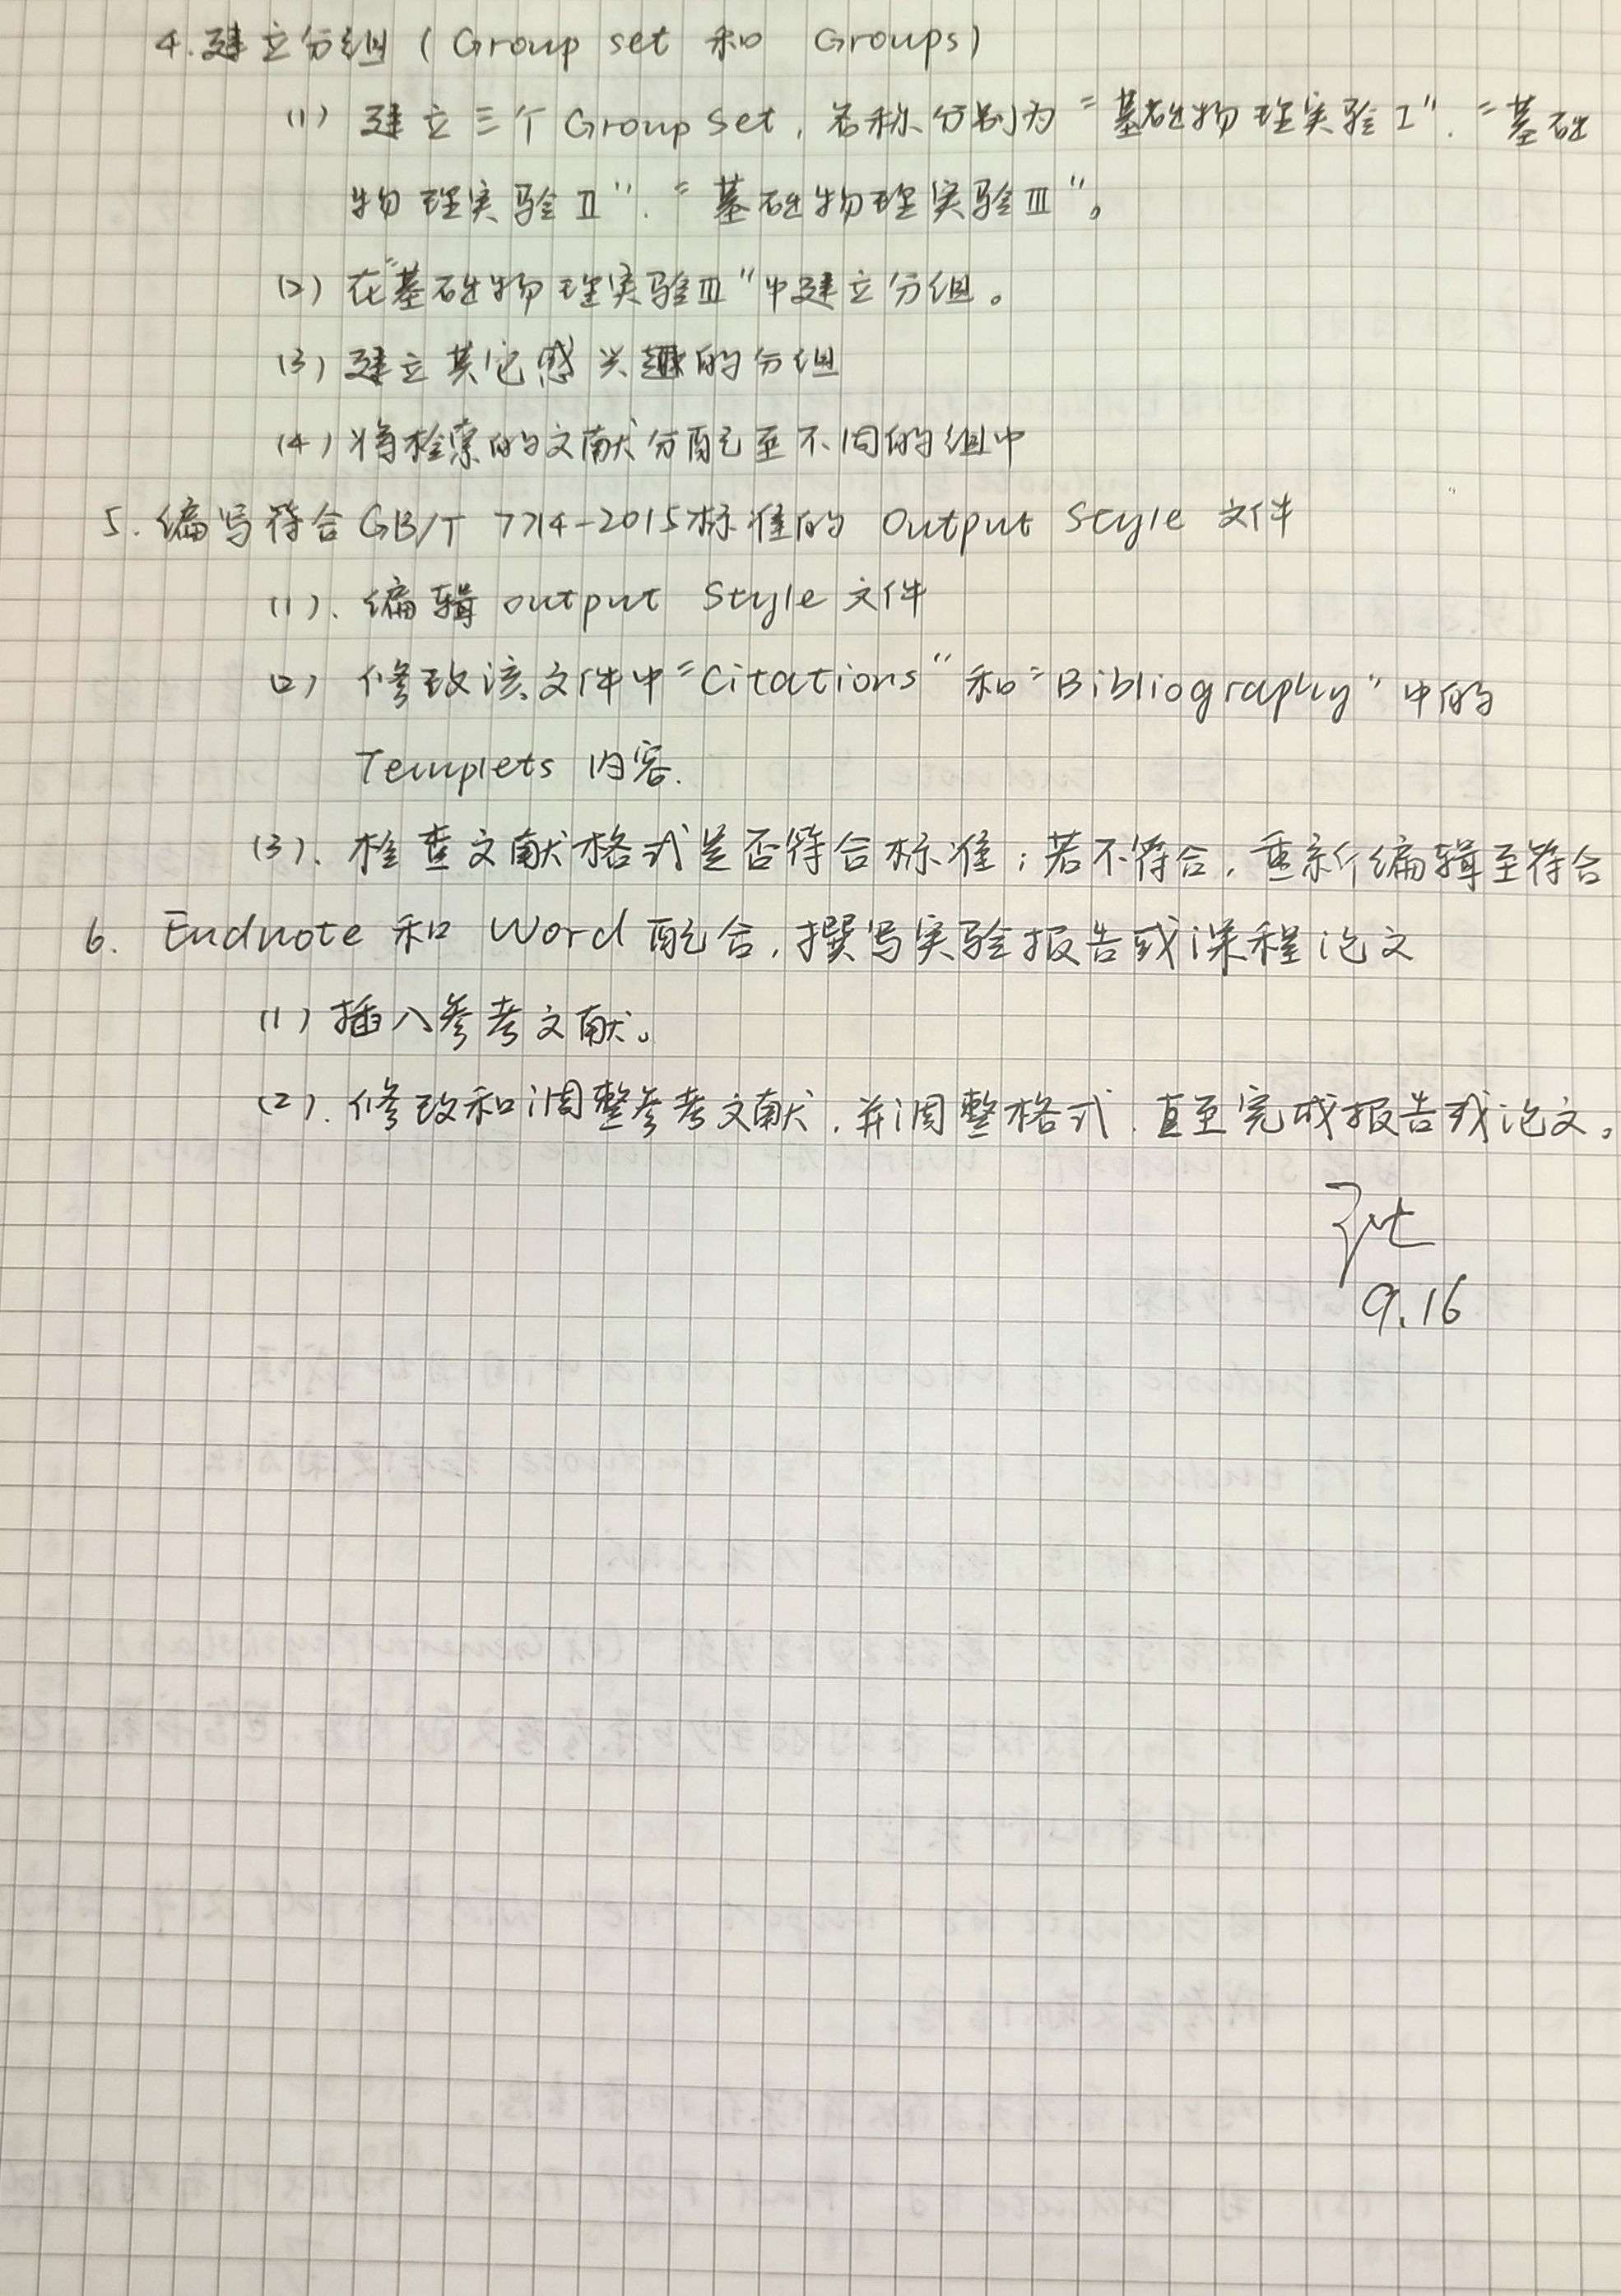
\includegraphics[width=0.8\textwidth]{img//preview2.jpg}
	\end{figure}

	
	
	\newpage
	\begin{center}
		\textbf{参考文献}
	\end{center}

[1] 中华人民共和国国家标准. 《信息与文献 参考文献著录规则》:GB/T 7714-
2015[S]. 2015.

[2] Thomson Reuters. Endnote X8 Basic[M]. Clarivate Analytics, 2014.

[3] Clarivate Analytics. Endnote Menus Reference Guide: Endnote Training[R]:
Clarivate Analytics, 2016.

[4] 童国伦,程丽华,张楷焄. EndNote \& Word 文献管理与论文写作[M]. 第二版. 
北京: 化学工业出版社, 2014.

[5] Clarivate Analytics. Editing Reference Types\&Styles:Windows: Endnote 
Support\&Training[R]: Clarivate Analytics, 2017.

[6] Clarivate Analytics. The Little Endnote How-to Book: Endnote Training[R]:
Clarivate Analytics, 2017.
	
\end{document}
